\documentclass[a4paper,12pt]{article}
\usepackage{caption}
\usepackage{subcaption}
\usepackage{graphicx}
\graphicspath{ {img/} }
\usepackage{fancyhdr}
\pagestyle{fancy}
\lhead{tqvj24}
\chead{}
\rhead{Image Processing Assignment}

\begin{document}

\section*{Discussion/detail of system design and choices made (5\%)}
\subsection*{System Design}
I wrote this script using Python 3.5.2, and OpenCv 3.1.0, to match the versions available on the DUDE PCs in the School.
Operation of the script is done via key presses, and output of the program is both visual in the main window, as well as various images being saved to disk, in the img\_out/ directory.
The main window displays one file ID at a time, with the top row being the w1 channel, and the bottom being w2. These are labelled, and labelling can be toggled by pressing the l key.
Full list of commands:
\begin{itemize}
    \item n - next image
    \item b - previous image
    \item l - toggle labels
    \item s - save the currently displayed w1 and w2 processed images
    \item x - exit
\end{itemize}
There are also boolean settings toward the top of the script, to allow for automatic saving of various images. \\
Processing of images is done in steps, with each step being a standalone method. All methods are documented and commented. The processing steps are as follows:
\begin{enumerate}
    \item Isolate and Compare
    \begin{enumerate}
        \item\textbf{Isolate} the worms from the background and border.
        \item\textbf{Compare} the isolated worms against the provided ground truth.
    \end{enumerate}

    \item Individualise and Save each worm
    \begin{enumerate}
        \item Run the \textbf{watershed} algorithm to mark worms with unique colours.
        \item Save each individual worm to disk, under img\_out/separated/ directory.
    \end{enumerate}

    \item Label each worm either dead or alive
    \begin{enumerate}
        \item Find the rotated bound box of each contour, and classify dead or alive depending on the width/height ratio of said box.
    \end{enumerate}
\end{enumerate}
Examples of what the above steps produce can be found under later sections. All images shown here are of A01, to clearly show the changes.

\subsection*{Choices Made}
As the images are saved as 16 bit but only really using 12 bits, when reading as 8 bit images the 4 most significant bits were lost, and the image was very dark (Figure 1), and so I read in the images as 16 bit, right shifted by 4 bits, and then converted to 8 bit. This ignores the 4 least significant bits, in favour of the 4 most significant bits. This results in a much more usable and bright image (Figure 2).\\
\begin{figure}[ht!]
    \centering
    \begin{subfigure}{0.5\textwidth}
        \centering
        
\includegraphics[width=0.8\textwidth]{A01_step0_unshifted.jpg}
        \caption{Loaded as 8 bit}
        \label{Figure 1}
    \end{subfigure}%
    \begin{subfigure}{0.5\textwidth}
        \centering
        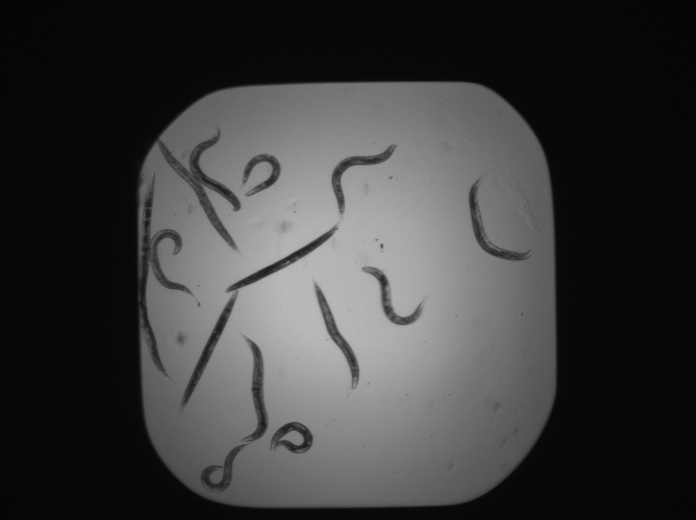
\includegraphics[width=0.8\textwidth]{A01_step0.jpg}
        \caption{Loaded as 16 bit and shifted}
        \label{Figure 2}
    \end{subfigure}
\end{figure}

% removing border via dialation (biggest contour didn't work because of clusters)
% threshold vs histogram equilisation
% comparison to ground truth (very high percentages because of big borders and empty spaces)
% detecting if dead or alive (isContourConvex was bad)

\section*{Evidence of the success of system in performing the specified task (5\%)}
\subsection*{Processing Steps}
% include images here of each step
% 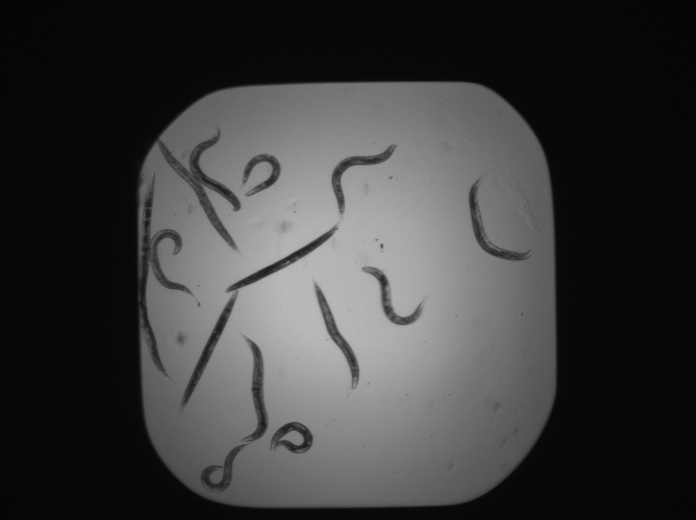
\includegraphics[width=0.95\textwidth]{A01_step0.jpg}  % for example

\centering{tqvj24}
\end{document}
